\documentclass[varwidth=true]{standalone}
\usepackage{tikz}
\begin{document}
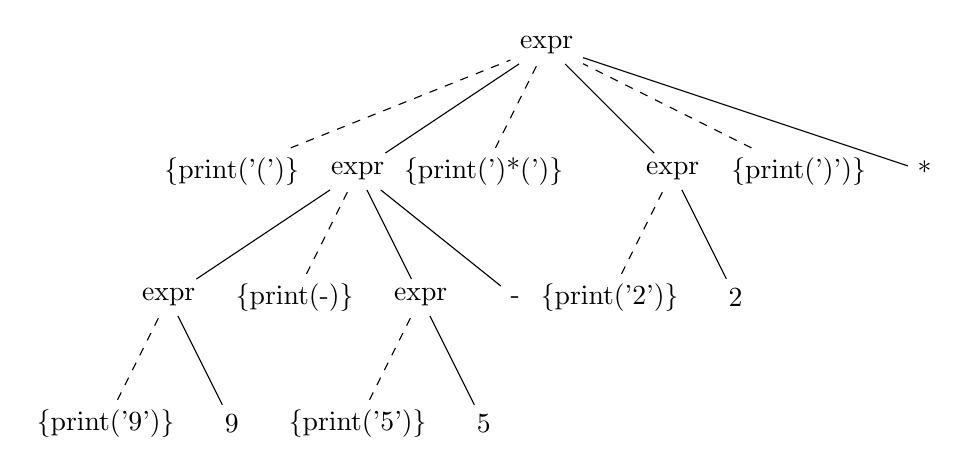
\begin{tikzpicture}[scale=0.8]
  \node (p9) at (-2, 0) {\{print('9')\}};
  \node (9) at (0, 0) {9};
  \node (p5) at (2, 0) {\{print('5')\}};
  \node (5) at (4, 0) {5};

  \node (e9) at (-1, 2) {expr};
  \node (p-) at (1, 2) {\{print(-)\}};
  \node (e5) at (3, 2) {expr};
  \node (-) at (4.5, 2) {-};
  \node (p2) at (6, 2) {\{print('2')\}};
  \node (2) at (8, 2) {2};

  \draw[dashed] (p9) -- (e9);
  \draw (9) -- (e9);
  \draw[dashed] (p5) -- (e5);
  \draw (5) -- (e5);

  \node (pob) at (0, 4) {\{print('(')\}};
  \node (e-) at (2, 4) {expr};
  \node (p*) at (4, 4) {\{print(')*(')\}};
  \node (e2) at (7, 4) {expr};
  \node (pcb) at (9, 4) {\{print(')')\}};
  \node (*) at (11, 4) {*};

  \draw (e9) -- (e-);
  \draw[dashed] (p-) -- (e-);
  \draw (e5) -- (e-);
  \draw (-) -- (e-);
  \draw[dashed] (p2) -- (e2);
  \draw (2) -- (e2);

  \node (e) at (5, 6) {expr};

  \draw[dashed] (pob) -- (e);
  \draw (e-) -- (e);
  \draw[dashed] (p*) -- (e);
  \draw (e2) -- (e);
  \draw[dashed] (pcb) -- (e);
  \draw (*) -- (e);
\end{tikzpicture}
\end{document}
